% !TeX encoding = UTF-8
% !TeX program = pdfLaTeX
% !TeX root = matlab-exercises-emaip.tex
% !TeX spellcheck = en_GB
\section{Fitting models to data}

Here is a set of exercises related to the lesson
on loading data into Matlab and fitting models to data.

\begin{ex}
Make the figure inserted below: \par
\noindent
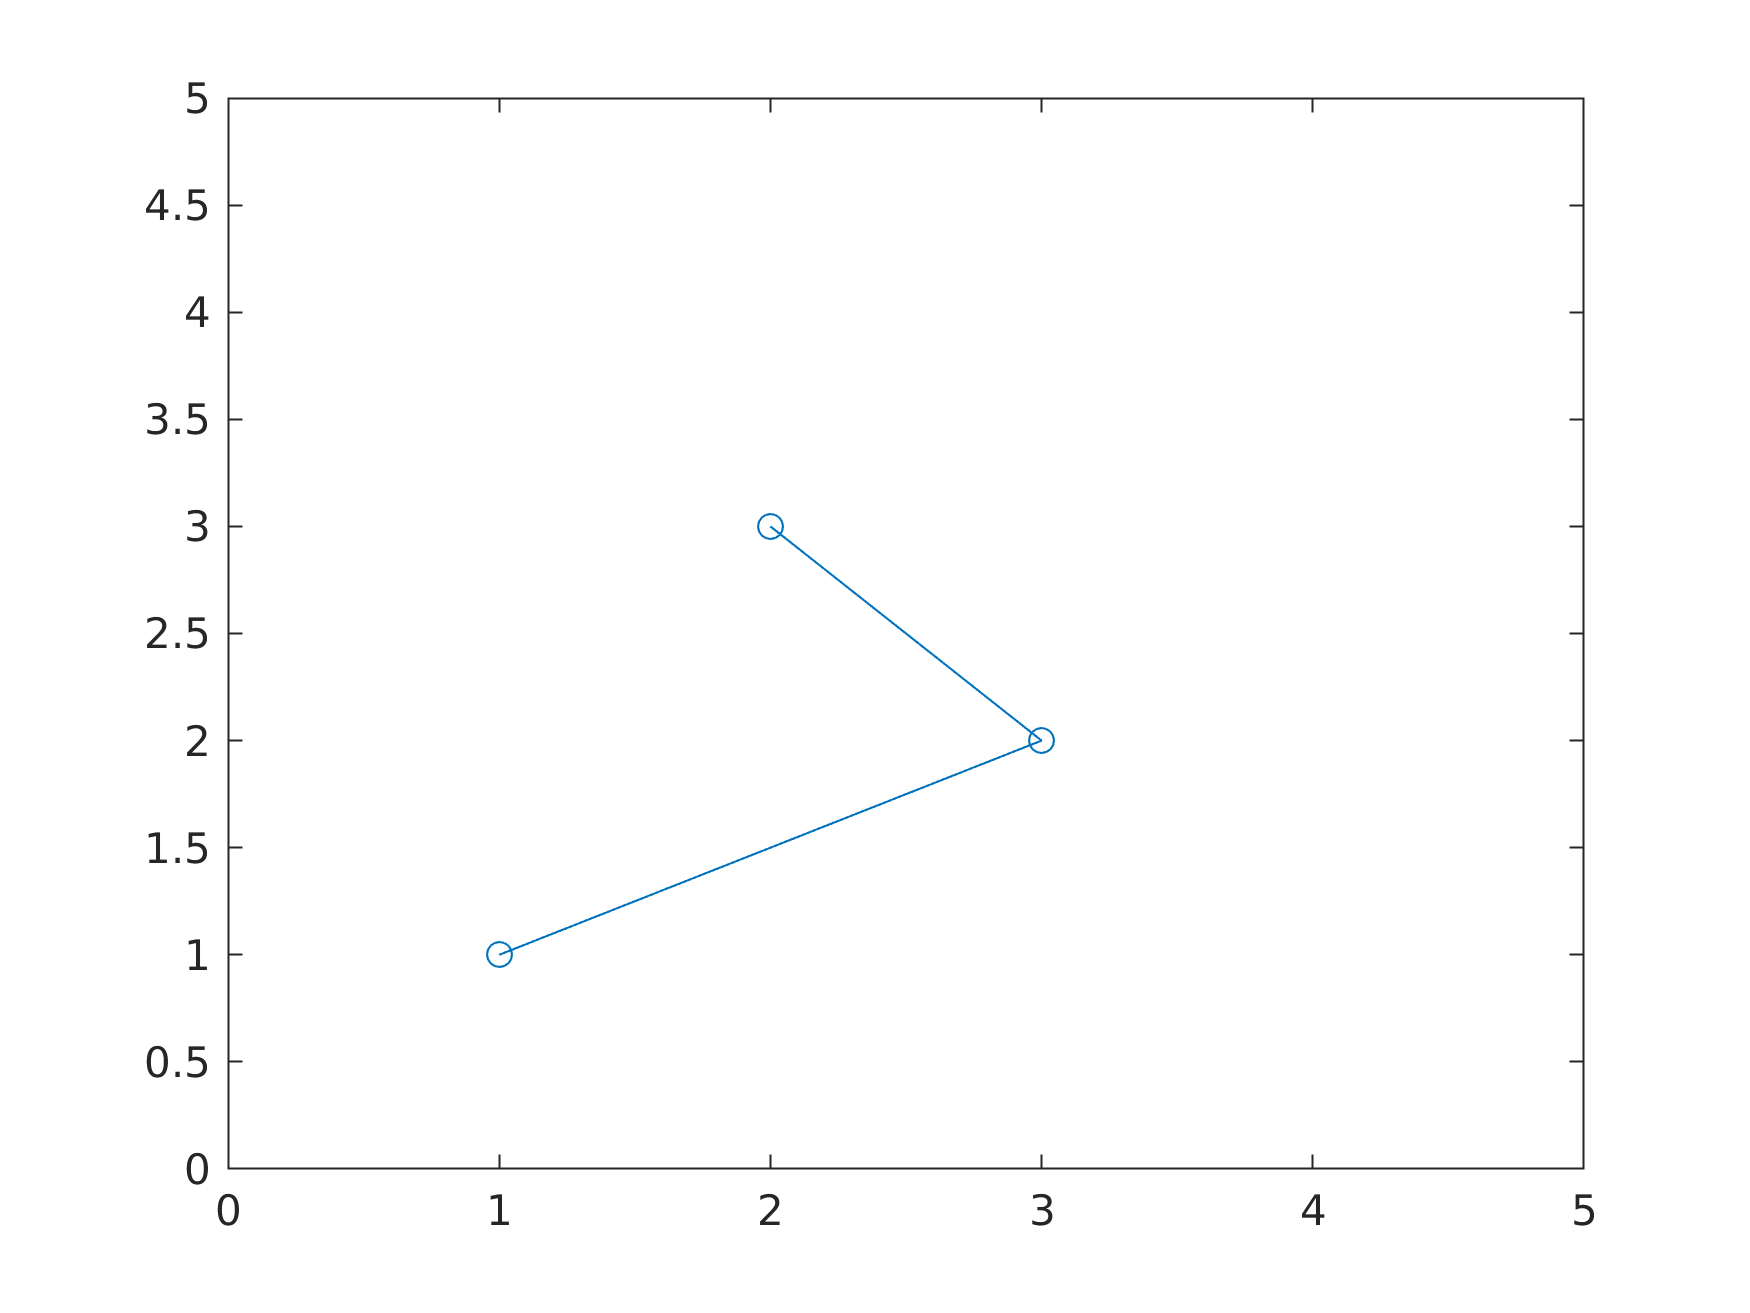
\includegraphics[width=8cm]{pic/plotting/basic_plotting_010.png}
\begin{hint}
The commands \verb!plot!, \verb!xlim! and \verb!ylim! can be useful.
\end{hint}
\begin{sol}
A solution is:
\begin{verbatim}
figure(1);
clf;
x = [1, 3, 2];
y = [1, 2, 3];
plot(x, y, '-o');
xlim([0, 5]);
ylim([0, 5]);
\end{verbatim}
\end{sol}
\end{ex}

\begin{ex}
Find a root of the function $f(x) = e^{-x} - x$.
\begin{hint}
The command \verb!fzero! can be useful.
\end{hint}
\begin{sol}
A solution is:
\begin{verbatim}
fh = @(x) exp(-x) - x
root1 = fzero(fh, 1)
\end{verbatim}
\end{sol}
\end{ex}

\begin{ex}
Find the minimum of the function $f(x) = e^x - 2x$.
\begin{hint}
The command \verb!fminsearch! can be useful.
\end{hint}
\begin{sol}
A solution is:
\begin{verbatim}
fh = @(x) -2x + exp(x);
fminsearch(fh, 1)
\end{verbatim}
\end{sol}
\end{ex}




\begin{ex}
Plot the functions $f(x) = e^x$ and $g(x) = 4x$ over the interval $x \in [-1, 3]$.
\begin{hint}
Define two function handles, one to each function.
Use the functions \verb!linspace!, \verb!hold on!, \verb!plot! and \verb!figure!.
\end{hint}
\begin{sol}
A solution is:
\begin{verbatim}
fh = @(x) exp(x);
gh = @(x) 4*x;
x = linspace(-1, 3);
figure(1);
clf;
hold on;
plot(x, fh(x));
plot(x, gh(x))
\end{verbatim}
\end{sol}
\end{ex}


\begin{ex}
Download the file \verb!test.csv! from this 
\href{https://raw.githubusercontent.com/henrikmidtiby/matlab-notes/master/code/loading_data/test.csv}{link}.
Load the data into matlab and plot the data.
Use the first column as $x$ values and the second column
as $y$ values.
\begin{hint}
\end{hint}
\begin{sol}
A solution is:
\begin{lstlisting}
% Download the datafile, this could also be done
% through the web browser.
url = 'https://raw.githubusercontent.com/henrikmidtiby/matlab-notes/master/code/loading_data/test.csv';
filename = 'test.csv';
outfilename = websave(filename, url);

% Load the data into matlab
data = dlmread(filename);
figure(1);
hold off;
% Plot data in column 1 (the x values) against the 
% data in column 2 (the y values).
%
plot(data(:, 1), data(:, 2));
\end{lstlisting}
\end{sol}
\end{ex}

\begin{ex}
Make the figure inserted below. Pay attention to the axes labels and the width of the plotted line. The visualized function is $f(x) = x^2 - x$. \par
\noindent
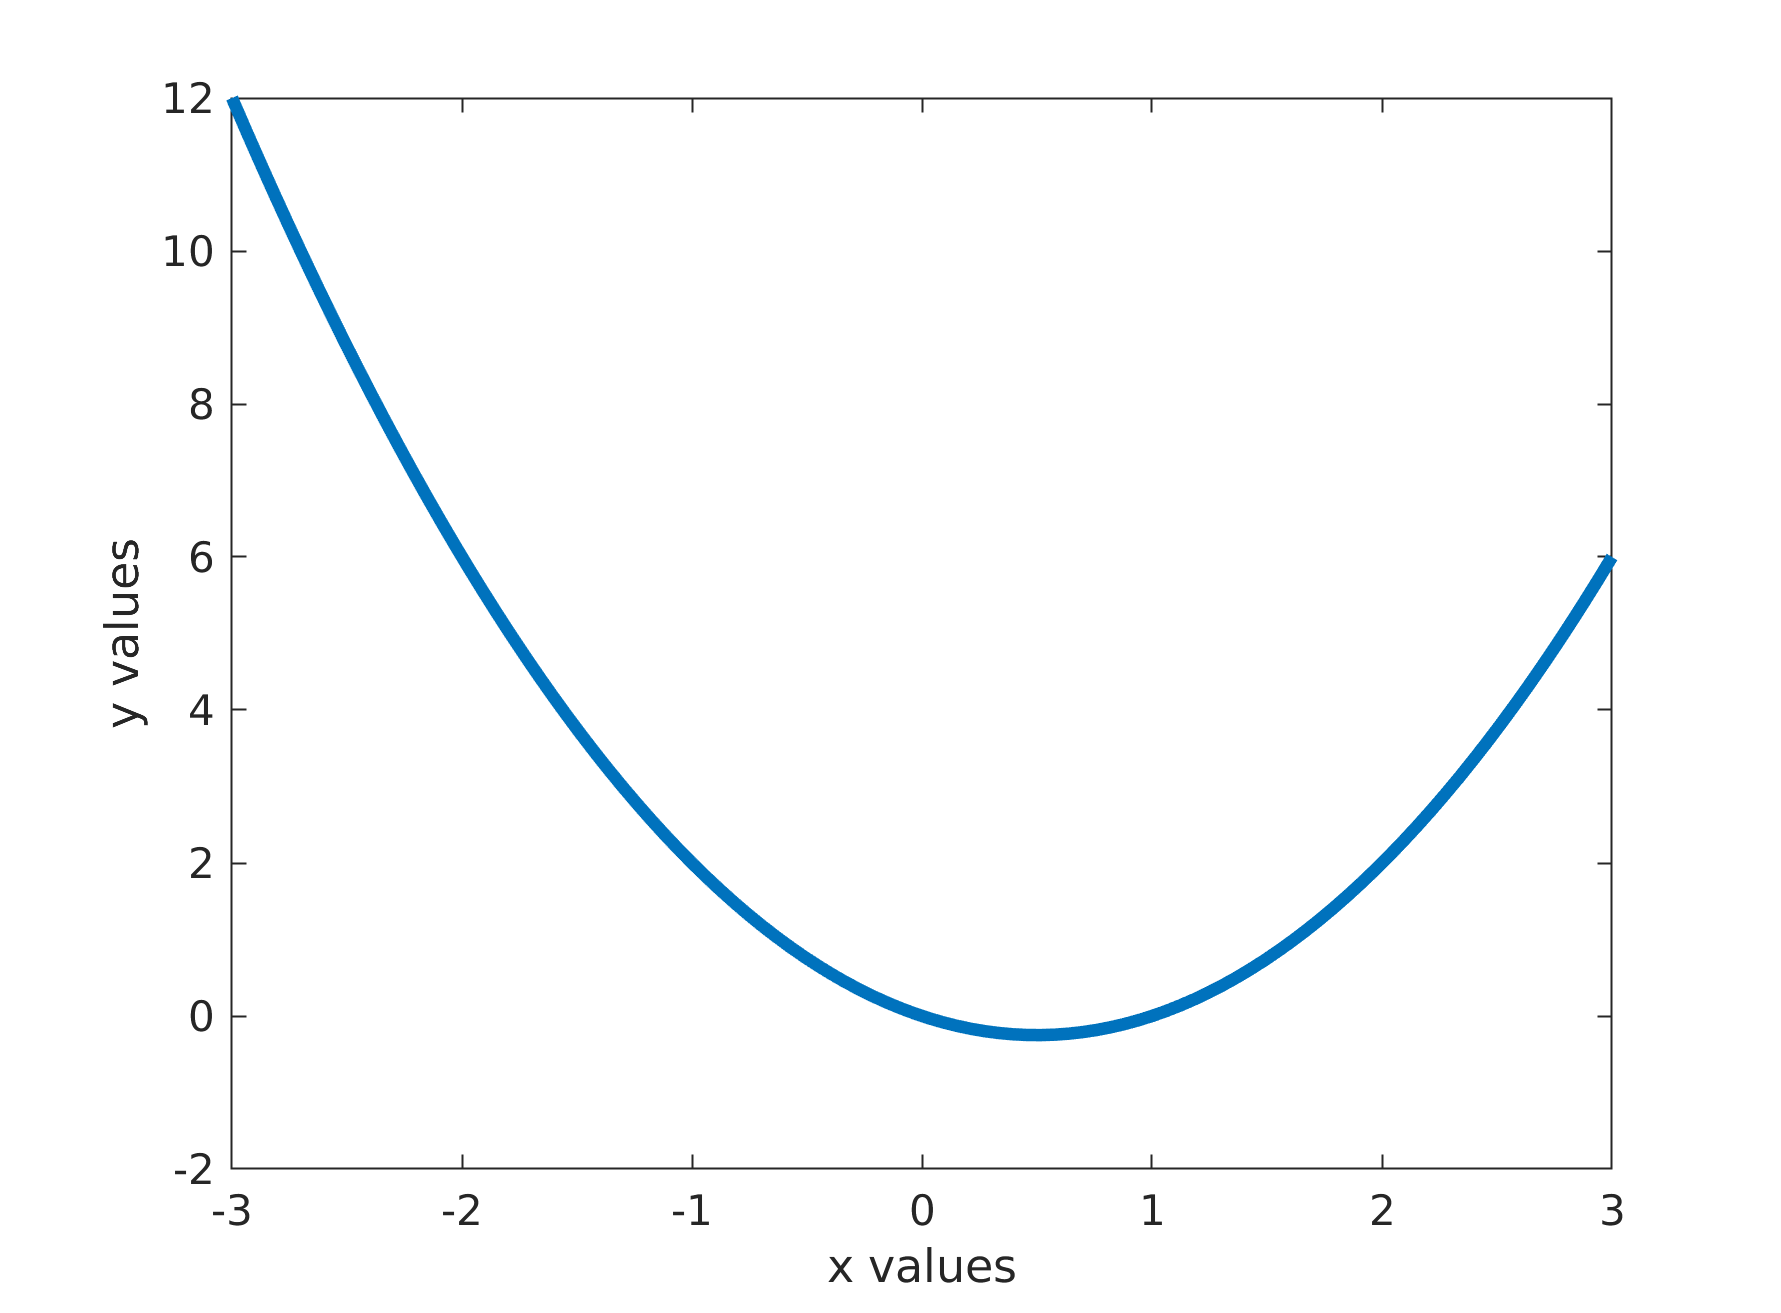
\includegraphics[width=8cm]{pic/plotting/basic_plotting_020.png}
\begin{hint}
The commands \verb!plot!, \verb!xlabel! and \verb!ylabel! can be useful.
\end{hint}
\begin{sol}
A solution is:
\begin{verbatim}
figure(1);
clf;
fh = @(x) -x + x.^2;
x = linspace(-3, 3);
plot(x, fh(x), 'LineWidth', 3);
xlabel('x values');
ylabel('y values');
\end{verbatim}
\end{sol}
\end{ex}


\begin{ex}
Find two numerical solutions to the equation
\[
e^{x} = 4x
\]
\begin{hint}
Write the equation on the form $f(x) = 0$ (collect all elements on the left hand side).
The command \verb!fzero! can be useful.
\end{hint}
\begin{sol}
A solution is:
\begin{verbatim}
% Plot functions (left hand side and right hand side 
% of the equation).
f = @(x) exp(x);
g = @(x) 4*x;
x = linspace(0, 2.5);
figure(1);
hold off;
plot(x, f(x));
hold on;
plot(x, g(x));

% Locate solutions / zeros
difference = @(x) f(x) - g(x);
root1 = fzero(difference, 0.3)
root2 = fzero(difference, 2.1)
\end{verbatim}
\end{sol}
\end{ex}



\begin{ex}
Solve the set of linear equations
\begin{align*}
1	& = 5x + 2y	\\
0	& = -x + y + 3z + 2v	\\
-10 	& = x + 3y - 4z + v	\\
0	& = -2x + 3z - 2v 
\end{align*}
\begin{hint}
Write the system of equations on matrix form $A \cdot \vec{x} = \vec{b}$.
\end{hint}
\begin{sol}
A solution is:
\begin{verbatim}
A = [5, 2, 0, 0; -1, 1, 3, 2; 1, 3, -4, 1; -2, 0, 3, -2];
b = [1; 0; -10; 0];
x = linsolve(A, b)
A * x
\end{verbatim}
\end{sol}
\end{ex}



\begin{ex}
Enter\label{exPlotDataToFitLinearModelTo}
the following values for $x$ and $y$ and plot the points.
Then describe the trend you are observing in the data.
\begin{verbatim}
x = [1, 2, 3, 5];
y = [4, 3, 2, 1];
\end{verbatim}
\begin{hint}
Use the \verb!plot! method.
\end{hint}
\begin{sol}
A solution is:
\begin{verbatim}
x = [1, 2, 3, 5];
y = [4, 3, 2, 1];
figure(1);
clf;
plot(x, y, 'o');
\end{verbatim}
From the plot I see that the $y$ values decreases as the $x$ values increases.
\end{sol}
\end{ex}

\begin{ex}
This\label{exPlotDataToFitLinearModelTo2}
exercise is a continuation of exercise \ref{exPlotDataToFitLinearModelTo}.\\
Implement a linear model $y = a \cdot x + b$ in matlab. 
The linear model should be defined like below, where P is a vector containing the 
model parameters $a$ and $b$.
\begin{verbatim}
model = @(x, P) <fill in stuff here>;
\end{verbatim}
\begin{hint}
The output of the model should match the output below.
\begin{verbatim}
>> model([1, 2, 3, 5], [-1, 5])
ans =
     4     3     2     0
\end{verbatim}
\end{hint}
\begin{sol}
A solution is:
\begin{verbatim}
model = @(x, P) P(1) * x + P(2);
\end{verbatim}
\end{sol}
\end{ex}

\begin{ex}
This \label{exPlotDataToFitLinearModelTo3}
exercise is a continuation of exercise \ref{exPlotDataToFitLinearModelTo2}.\\
Implement a method that calculates the squared error
between the model and observations.
\[
\text{squared error} = \sum_i \left(y_i - \text{model}(x_i)\right)^2
\]
Assume that the $x$ and $y$ values are saved in the variables 
\verb!x! and \verb!y! respectively.
\begin{verbatim}
model_error = @(P) <fill in stuff here>;
\end{verbatim}
\begin{hint}
The \verb!sum! function is helpful.
\end{hint}
\begin{sol}
A solution is:
\begin{verbatim}
>> x = [1, 2, 3, 5];
>> y = [4, 3, 2, 1];
>> model = @(x, P) P(1) * x + P(2);
>> model_error = @(P) sum((y - model(x, P)).^2);
>> squared_error = model_error([-1.2, 5])
squared_error =
    4.5600
\end{verbatim}
\end{sol}
\end{ex}

\begin{ex}
This exercise is a continuation of exercise \ref{exPlotDataToFitLinearModelTo3}. \\
Minimize the squared error, defined in exercise \ref{exPlotDataToFitLinearModelTo3} 
and then plot the model with the 
found parameter values along with the original data.
\begin{hint}
You can try to minimize the function manually by calling it with different 
parameters and then adjust the parameters so that the function value
is reduced. It could look like this.
\begin{lstlisting}
>> squared_error = model_error([-1.2, 5])
squared_error = 4.5600
>> squared_error = model_error([-1.2, 4.5])
squared_error = 8.7600
>> squared_error = model_error([-1.2, 5.5])
squared_error = 2.3600
>> squared_error = model_error([-1.25, 5.5])
squared_error = 3.1875
>> squared_error = model_error([-1.15, 5.5])
squared_error = 1.7275
\end{lstlisting}


The \verb!fminsearch! function is helpful, it should converge to 
the proper solution independent of the initial guess.
The solution contains the following values $-0.7429$ and $4.5429$.
\end{hint}
\begin{sol}
A solution is:
\begin{verbatim}
x = [1, 2, 3, 5];
y = [4, 3, 2, 1];
model = @(x, P) P(1) * x + P(2);
model_error = @(P) sum((y - model(x, P)).^2);
P = fminsearch(model_error, [4, 2])

xvals = linspace(0, 6);
figure(1);
clf;
hold on;
plot(x, y, 'o');
plot(xvals, model(xvals, P));
\end{verbatim}
\end{sol}
\end{ex}



\begin{ex}
Plot the three functions given below in the same plot.
\[
f(x) = \frac{1}{x + 1} \qquad \qquad g(x) = \frac{1}{x + 3} \qquad \qquad h(x) = \frac{1}{(x + 1)(x + 3)}
\]
Do the functions have something in common?
\begin{hint}
Look at the discontinuities of the functions. Where are they placed?
\end{hint}
\begin{sol}
A solution is:
\begin{verbatim}
fh = @(x) 1 ./ (x + 1);
gh = @(x) 1 ./ (x + 3);
hh = @(x) 1 ./ ((x + 1) .* (x + 3));
x = linspace(-5, 1, 1000);
figure(1);
clf; 
hold on;
plot(x, fh(x));
plot(x, gh(x));
plot(x, hh(x));
ylim([-4, 4]);
\end{verbatim}
\end{sol}
\end{ex}

\begin{ex}
Given the three functions below:
\[
f(x) = \frac{1}{x + 1} \qquad \qquad g(x) = \frac{1}{x + 3} \qquad \qquad h(x) = \frac{1}{(x + 1)(x + 3)}
\]
Plot $h(x)$ and a linear combination of $f(x)$ and $g(x)$ in the same plot.
Adjust the coefficients of $f(x)$ and $g(x)$, so that the two plotted functions 
becomes as similar as possible.
\begin{hint}
An example of a linear combination of $f(x)$ and $g(x)$ is
\[
2 \cdot f(x) + 3 \cdot g(x)
\]
\end{hint}
\begin{sol}
A solution is:
\begin{verbatim}
fh = @(x) 1 ./ (x + 1);
gh = @(x) 1 ./ (x + 3);
hh = @(x) 1 ./ ((x + 1) .* (x + 3));
figure(2);
clf; 
hold on;
plot(x, 0.5*fh(x) - 0.5*gh(x));
plot(x, hh(x), 'LineStyle', '- -', 'LineWidth', 3);
ylim([-4, 4]);
\end{verbatim}
\end{sol}
\end{ex}



\begin{ex}
Use the debugger to examine the \verb!binary_log! function.
\begin{enumerate}
\item Open the file \href{https://raw.githubusercontent.com/henrikmidtiby/matlab-notes/master/code/debugger_example_binary_log/binary_log.m}{binary.log}
\item	Insert a \verb!fprintf! statement in line 3, that prints the input arguments given to the function.
\item	Insert a breakpoint (red circle next to the line numbers) at the start of the function "\verb!binary_log!".
\item	Call the function as "\verb!binary_log(8)!" and step through the method using the debugger.
\item	Insert a comment in the function that explains what the while loop in line 6--9 is doing.
\item	Call the function as "\verb!binary_log(0.25)!" and step through the method using the debugger.
\item	Insert a comment in the function that explains what the while loop in line 11--14 is doing.
\end{enumerate}
\begin{hint}
Log rules to be aware of
\[
\log_2(2 \cdot a) = 1 + \log_2(a) \\
\log_2(a / 2) = -1 + \log_2(a)
\]
\end{hint}
\begin{sol}
Lines 6--9 applies the rule $\log_2(2 \cdot a) = 1 + \log_2(a)$ until $a$ is less than 2.

Lines 11--14 applies the rule $\log_2(a / 2) = -1 + \log_2(a)$ until $a$ is greater than or equal to 1.
\end{sol}
\end{ex}
 